\section{Booth Function}
\label{sec:app:test:booth}

  The Booth function is a quadratic test problem used in the optimization field,
  specifically tailored for algorithms that handle two-dimensional search spaces.

  \begin{definition}[Booth Function]
    \label{def:app:test:booth}
    The \emph{Booth function}, \(f: \mathbb{R}^2 \rightarrow \mathbb{R}\), is 
    defined as:

    \begin{equation}
    \label{eq:app:test:booth}
      f(x,\, y) = (x + 2y - 7)^2 + (2x + y - 5)^2
    \end{equation}
    
    where:
    \begin{itemize}
      \item \(x,\, y \in \mathbb{R}\) represent the decision variables.
    \end{itemize}
  \end{definition}

  The global minimum of the Booth function is \(f(1, 3) = 0\).
  The function is usually constrained to the square \([-10, 10]^2\).
  A contour plot and a surface plot of the Booth function are illustrated in 
  \vref{fig:app:test:booth}.

  \begin{figure}[ht!]
    \centering
    \begin{subfigure}[b]{0.45\textwidth}
      \centering
      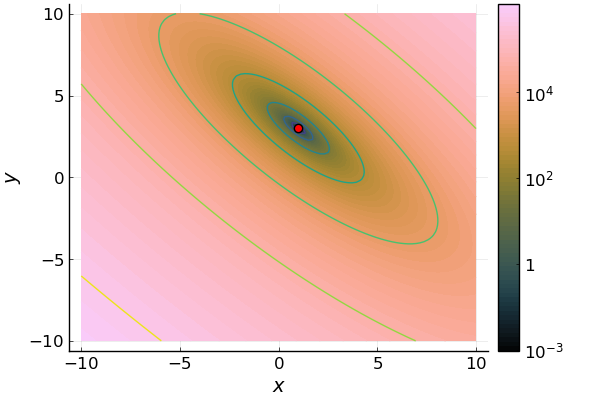
\includegraphics[width=\textwidth]{img/test_functions/booth_contour.png}
    \end{subfigure}
    \hfill
    \begin{subfigure}[b]{0.45\textwidth}
      \centering
      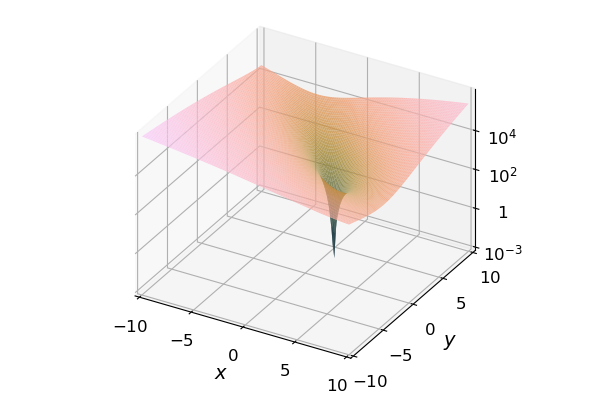
\includegraphics[width=\textwidth]{img/test_functions/booth_surface.png}
    \end{subfigure}
    \caption{Booth Function}
    \label{fig:app:test:booth}
  \end{figure}
